\documentclass[../catalog.tex]{subfiles}

\begin{document}

Throughout the previous chapters we have seen how to continuously
maintain high-arity joins with robust, adaptive performance and within
a constant memory footprint, using delta queries and worst-case
optimal join algorithms. Neither of these measures had a significant
negative impact on absolute query performance. Still, we have somewhat
overcorrected, at the expense of redundancies in the overall
dataflow. Apart from the attribute indices, we have ignored almost all
opportunities for sharing resources between dataflows.

Query dataflows consume a number of resources over their entire
lifetime, which might be measured in minutes or hours for interactive
sessions, but in days, weeks, months, or even years for dataflows
between backend services. The primary resource consumed by a dataflow
element is space to (potentially) buffer and index its inputs. We
refer to this as \emph{operator state}. To a lesser extent dataflow
elements themselves incur some marginal costs both in space, for
maintaining a representation of the dataflow graph, and in time,
because additional operators need to receive and process progress
information. Naturally, sharing neither indexed operator state, nor
dataflow elements, limits the number of clients we can support
concurrently.

\subsection{Example}

Consider again a scenario of many analysts concurrently interacting
with the same data streams. Many of them will be interested in a
common subset of data, e.g. users that are currently active in Europe,
but will impose some additional constraints depending on their
respective tasks at hand. A more concrete example might be the comment
stream from previous chapters:

\begin{verbatim}
[(comment ?comment ?place ?person ?ip ?content ...)

 [?comment :comment/creation-date ?creationDate]
 [?comment :comment/creator ?person]
 [?comment :comment/ip ?ip]
 [?comment :comment/browser ?browser]
 [?comment :comment/content ?content]
 [?comment :comment/place ?place]]
\end{verbatim}

We have multiple analysts, each interested only in comments from a
specific location. For an analyst interested in comments originating
in Zurich, a query might look like the following:

\begin{verbatim}
[:find ...
 :where
 (comment ?comment ?place ...)
 [?place :place/name "Zurich"]]
\end{verbatim}

A similar situation naturally arises when implementing data access
policies, which forces clients to only work with certain subsets of
all available data. Datalog makes it possible to succintly express
even complex, property-based policies. A set of rules describing a
simplified, role-based access control scheme might look like:

\begin{verbatim}
[:find ?document ?content
 :where
 (access? <client-id> ?document)
 [?document :document/content ?content]]

[[(access? ?client ?document)
  [?client :client/role ?role]
  (role-access? ?role ?document)]

 [(role-access? ?role ?document)
  [?role :role/access? ?document]]
 
 [(role-access? ?role ?document)
  [?child :role/super ?role]
  (role-access? ?child ?document)]]
\end{verbatim}

Intuitively we might point out that recursively re-deriving the
\texttt{role-access?} relation for each client seems wasteful.

\subsection{Sharing Dataflows}

In general, given $n$ analysts, we can service their queries in a few
different ways.

\textbf{Shared Nothing} We create $n$ indepedent dataflows, sharing
only the base relation indices. This gives us the greatest freedom to
pick the best possible plans for each individual analyst, for example
making use of the worst-case optimal join framework covered in
chapters \ref{technique-wco} and \ref{case-join-ordering}. On the
other hand, all of those $n$ dataflows will perform a lot of redundant
work and incur significant overheads, deriving $n$ copies of the
\texttt{comment} relation.

\textbf{Shared Trunk} Differential's \emph{arrangements} allow us to
re-use materialized relations between dataflows. We could therefore
create a single dataflow deriving the \texttt{comment} relation, on
top of which $n$ specialized dataflows will be only be responsible for
implementing the specific additional joins requested by each
analyst. Because arrangements materialize tuples into sorted batches,
doing so will cost extra storage proportional in the size of the
`comment` relation, on top of the storage taken up by base relations
(c.f. \ref{case-join-state}).

Sharing a common part of the dataflow (a \emph{shared trunk}) avoids
redundant derivations of the \texttt{comment} relation and
significantly reduces the total number of dataflow elements created (a
super-linear reduction in case of delta-queries), at the cost of some
extra storage — seemingly a fine trade-off!

On the other hand, materializing a shared trunk fixes the space of its
possible implementations. In particular (as touched on in
\ref{case-eagerness}) it prevents us from exploiting highly selective
constraints provided by individual analysts to cut down on the number
of tuples produced by each flow. In the specific case of the
\texttt{comment} relation, this might not be a problem, as the number
of tuples produced during its derivation is proportional to the number
of comments in the system. For other relations (for example the
transitive graph induced by the \texttt{:person/knows} relation) it
might lead to catastrophic plans.

Whenever we are considering to build multiple dataflows off of a
shared trunk, we must therefore estimate whether the shared trunk is
\emph{sufficiently selective}.

Here we are again faced with what is essentially the defining
trade-off of this work: increased specialization opens optimization
potential, whereas increased generalization opens potential for
resource re-use. After all our work to avoid heuristics and
cardinality estimation, we would not want to re-introduce an element
of unpredictability into the behaviour of our system.

Computing multiple redundant instance of a plan where worst-case
optimal execution improves the asymptotic complexity can still be
significantly cheaper than sharing the sub-optimal plan. Additionally,
once we've made the decision to share a flow, we must commit to
maintaining it for as long as any dependent flows are active.

Consistent with our robustness goal, we therefore want to err on the
side of caution at the expense of reduced best-case
scalability.

\subsection{Multi-Tenant Dataflows}

In some situations, an additional implementation strategy might be
available to us: we can model multi-tenancy within the data plane
itself. Recall the query from earlier:

\begin{lstlisting}[language=datalog, style=colorlog]
[:find ...
 :where
 (comment ?comment ?place ...)
 [?place :place/name "Zurich"]]
\end{lstlisting}

As a first step, we will re-write this query, replacing the explicit
filter by a parameter input, drawn from an additional parameter
attribute.

\begin{lstlisting}[language=datalog, style=colorlog]
[:find ...
 :where
 (comment ?comment ?place ...)
 [?place :place/name ?name-filter]
 [_ :parameter/place-name ?name-filter]]
\end{lstlisting}

This is useful in an of itself, because it gives us the ability to
update the filter parameter (with updated results derived
incrementally as usual), without registering separate queries. Once a
query is parameterized in this way, we can allow multiple concurrent
users to interact with the same parameter collection. Of course we
must then make sure to isolate users from each other and route results
correctly.

In this (admittedly simple) situation we can use a single dataflow for
all $n$ analysts, while still being able to move the
\texttt{:place/name} constraints into the same, worst-case optimal
query plan. Still, real-world use cases (such as the access control
policy from above) can already benefit from multi-tenant
parameterization.

We find precedence for this approach in the NiagaraCQ system by
\cite{chen2000niagaracq}.

\begin{quote}
NiagaraCQ implements sharing even when operators differn in certain
constants, by implementing the operators using relational joins
against the table of constants \cite{chen2000niagaracq}.

\cite{hirzel2014catalog}
\end{quote}

It is also reminiscent of more recent work on partially-stateful,
multi-tenant dataflow systems by \cite{gjengset2018noria}.

\subsection{Identifying Opportunities for Re-use}

Of course, re-use via parameterized, multi-tenant dataflows is not
possible if users request different conjunctions. Finding common
sub-structures across query plans that would be suitable for either of
the approaches outlined above is in general a very computationally
intensive problem.

Declarative languages allow for simplified, pragmatic
approach. Instead of arbitrary re-use across all clauses in all rules,
we only consider re-use at rule boundaries.

To facilitate this, each rule should be given a unique name. We can
further break this down and give unique names to all conjunctions,
e.g. by creating separate rules for the different branches of an
\texttt{or} clause automatically. Additionally, we can split off plan
stages that do not affect the underlying joins, such as projections,
transformations, and aggregations.

\subsection{Re-Use And Worst-Case Optimal Dataflow Joins}

The worst-case optimal join operator outlined in chapter
\ref{case-join-ordering} warrants special consideration
w.r.t. resource sharing.

First, most such algorithms (and in particular our implementation,
c.f. chapter \ref{impl-hector}) assume that participating relations
are available, indexed by each possible subset of their bound
symbols. For a binary relation $(e,v)$ two indices would have to be
maintained (one from $e$ to $v$, and one reverse index). For a ternary
relation, e.g. $(a,b,c)$, already six indices are required.

We therefore, by default, break derived n-ary relations down into
their base relations. Re-using n-ary relations via a Differential
arrangement would force us to create the additional required indices
on the fly.

Leaving aside the considerations from above, re-use of derived binary
relations (e.g. \texttt{(access?  ?user ?document)}) is possible via
the same indexing structures used for base relations. Within the
dataflow model, index arrangements do not need to distinguish whether
they are being fed by external inputs or from a derived relation.

\subsection{Other Strategies}

Again from \cite{hirzel2014catalog} we learn that

\begin{quote}
YFilter implements sharing between applications written in a subset of
XPath by compiling them all into a combined NFA [Diao et al. 2002].
\end{quote}

Similar NFA-based approaches can be found in the literature on complex
event processing (e.g. \cite{agrawal2008}). While such methods are
available to us in Timely Dataflow (e.g. via the built-in
\texttt{StateMachine} operator), they do not fit cleanly into the
relational model implemented by 3DF and Differential Dataflow. The
question of whether the two approaches can be combined in a sensible
way is left for future inquiry.

\subsection{Evaluation}

We evaluated the performance of different re-use strategies with the
following scenario. A constant load of 500 tuples per second was
generated, simulating sensor measurements reported by different
devices. Every second of the experiment, ten new clients were
introduced using one of three strategies:

\begin{enumerate}
  \item 
\end{enumerate}

\begin{figure}[h!]
  \begin{subfigure}{1.0\textwidth}
    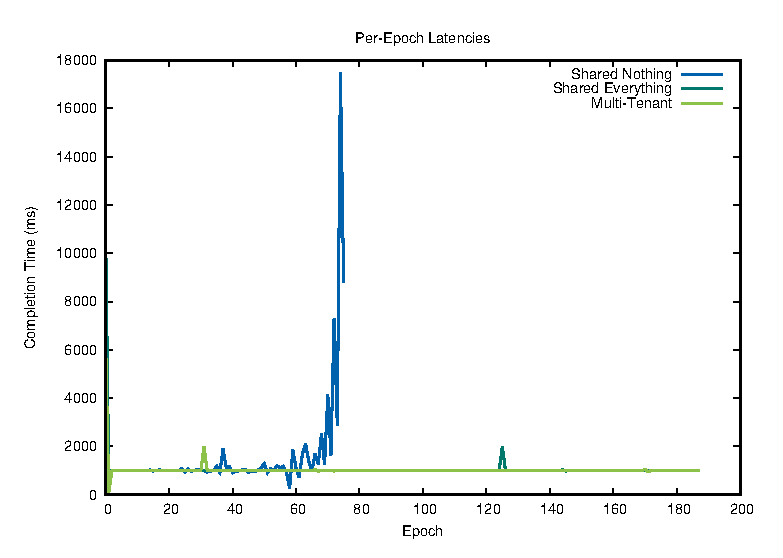
\includegraphics[width=1.0\linewidth]{results/multitenant_w1_p1/times}
    \caption{Single Worker}
  \end{subfigure}
  \begin{subfigure}{1.0\textwidth}
    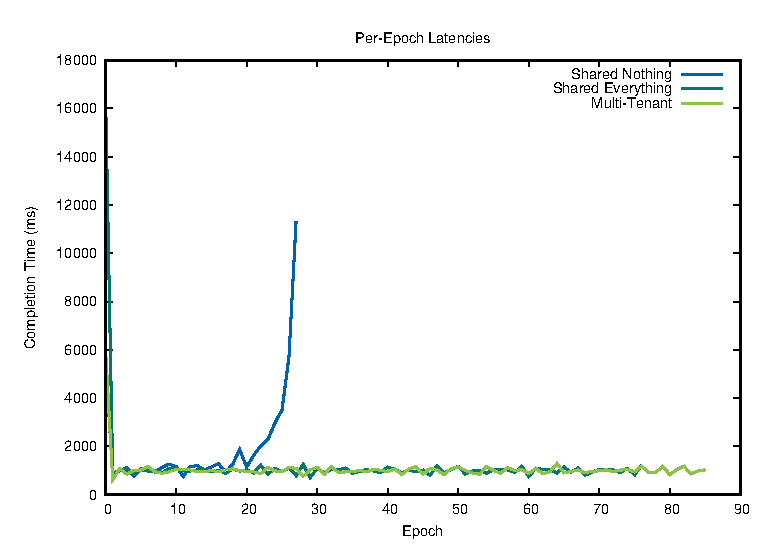
\includegraphics[width=1.0\linewidth]{results/multitenant_w1_p3/times}
    \caption{Three Distributed Workers}
  \end{subfigure}

  \caption{Per-Epoch Latencies}
\end{figure}

\end{document}
